\documentclass[12pt,a4paper]{article}
\usepackage{amsmath,amssymb,amsthm,bm}
\usepackage{geometry}
\geometry{margin=2.5cm}
\usepackage{hyperref}
\usepackage{booktabs}
\usepackage{array}
\usepackage{xcolor}
\usepackage{graphicx}
\usepackage{longtable}

\newcommand{\CMSTG}{\textsc{cmstg}}
\newcommand{\Psibar}{\bar\Psi}
\newcommand{\Feff}{F_{\rm eff}}
\newcommand{\Geff}{G_{\rm eff}}
\newcommand{\Lbare}{\Lambda_{\rm bare}}
\newcommand{\Lz}{\Lambda_0}
\newcommand{\Mpl}{M_{\rm Pl}}
\newcommand{\thetastar}{\theta_*}
\newcommand{\rs}{r_s}

\title{\textbf{Curvature-Memory Scalar-Tensor Gravity:\\
       Framework, Field Equations, and Cosmological Consistency}}
\author{Christopher~R.~B.~Wilson\thanks{E-mail: \texttt{C.Isomorph@gmail.com}. Independent researcher.}}
\date{2026}

\newcommand{\keywords}[1]{\par\noindent\textbf{Keywords:} \textit{#1}\par\bigskip}

\begin{document}
\maketitle

\begin{abstract}
We present the complete framework of Curvature-Memory Scalar-Tensor Gravity
(\CMSTG): a covariant scalar-tensor extension of general relativity in which
the scalar field $\Psi$ encodes retarded curvature history through a non-minimal
coupling $\Lz\Psi^2 R$ to the Ricci scalar. We derive the Euler--Lagrange and
modified Friedmann equations, establish the GR-recovery conditions, reduce the
theory to the FLRW cosmological background, and demonstrate canonical
quantization at free-field level. The Phase~1 canonical action with locked
parameters $\Lz = 0.003\,\Mpl^{-2}$, $\Psibar = 2.62\,\Mpl$, and effective
gravitational coupling $\Feff = (1 + 2\Lz\Psibar^2)/2 = 0.521$ is tested
against nine precision datasets: BAO full-covariance refit (BOSS+eBOSS+DESI~Y1),
CMB TT/TE/EE power spectra (Planck plikHM), RSD growth rate $f\sigma_8$,
non-linear structure growth $\sigma_8$, gravitational wave speed, Solar System
PPN constraints, and dark energy equation of state. All tests pass at current
observational precision. The effective gravitational coupling $\Geff/G =
1 - 15\,\mathrm{ppm}$ at $\Lz = 0.003$, placing \CMSTG\ observationally
degenerate with $\Lambda$CDM at the $10^{-5}$ level; the coupling is unconstrained
by current data with an estimated detection threshold at $\Lz \sim 0.05$.
The one residual is a $2.77\sigma$ tension with DESI~Y1 BAO, demonstrated
in a companion paper to be a structural floor not reducible within the
\CMSTG\ action class.
\end{abstract}

\keywords{scalar-tensor gravity; dark energy; baryon acoustic oscillations; CMB; modified gravity; cosmological perturbations}

\tableofcontents
\bigskip

% ─────────────────────────────────────────────────────────────────────────────
\section{Introduction}
\label{sec:intro}

General Relativity (GR) provides an extraordinarily accurate description of
spacetime at solar and astrophysical scales. At galactic and cosmological
scales, however, GR requires three auxiliary postulates---cold dark matter, a
cosmological constant $\Lambda$, and slow-roll inflation---none of which have
been detected directly in controlled laboratory settings. Each is introduced
to match specific observations rather than derived from deeper first principles.

The theoretical landscape of scalar-tensor gravity is rich. Brans--Dicke
theory~\cite{BransDicke1961} introduces a scalar $\phi$ coupled to $R/\phi$
with no dynamics; observationally, the Brans--Dicke parameter $\omega_{\rm BD}
> 40{,}000$ (Cassini bound~\cite{Bertotti2003}) pushes the scalar to be
dynamically irrelevant. $f(R)$ theories~\cite{Sotiriou2010} are equivalent to
Brans--Dicke with $\omega_{\rm BD} = 0$ and a potential, constrained by
the same tests. The general Horndeski class~\cite{Horndeski1974,Kobayashi2011}
encompasses all covariant scalar-tensor theories with second-order field
equations, including Galileon models~\cite{Nicolis2009} and beyond-Horndeski
theories~\cite{Gleyzes2015}. A key observational discriminant for any scalar-tensor
theory post-GW170817 is the gravitational wave speed: the multi-messenger
bound $|c_T/c - 1| < 7\times10^{-16}$~\cite{Abbott2017,Creminelli2017}
eliminates all Horndeski actions with non-trivial $G_5$ coupling.

Separately, the DESI Year~1 BAO measurements~\cite{DESI2024} report a
$\sim2.8\sigma$ preference for a dynamical dark energy equation of state
$(w_0, w_a) \neq (-1, 0)$ that is in tension with the Planck $\Lambda$CDM
prediction. This motivates the study of whether minimal scalar-tensor extensions
can accommodate or resolve the tension.

\emph{Curvature-Memory Scalar-Tensor Gravity} (\CMSTG) proposes that the
geometry of spacetime is governed not solely by local energy-momentum but also
by retarded curvature history encoded in a scalar field $\Psi$. The field
$\Psi$ satisfies a Klein--Gordon equation sourced by the Ricci scalar $R$, with
retarded boundary conditions selecting the unique causal solution: each past
curvature event contributes according to its causal influence, attenuated by
the field mass. The resulting theory is covariant, belongs to the Horndeski
class with $G_4 = (M_{\rm Pl}^2 + 2\Lz\Psi^2)/2$ and $G_5 = 0$
(ensuring $c_T = c$ exactly), contains GR as a strict limit, and admits
canonical quantization. The UV structure---one-loop finiteness, Ward identity
protection of the graviton sector, and an asymptotic freedom fixed point at
$\Lz = 0$---is established in a companion paper (Paper~III of this series~\cite{WilsonPaperIII}).

This paper develops the classical and free-field-quantized framework and
tests its cosmological predictions against precision data. The principal
result is that \CMSTG\ with the Phase~1 canonical action
\begin{equation}
  S_{\rm P1} = \int\!d^4x\,\sqrt{-g}\,\Bigl[
    \tfrac{1+2\Lz\Psi^2}{2}\,R
    - \tfrac{1}{2}(\partial\Psi)^2
    - \tfrac{1}{2}m_0^2\Psi^2
  \Bigr] + S_{\rm SM}
  \label{eq:phase1-action}
\end{equation}
is consistent with all current precision cosmological datasets at the
$10^{-5}$ level of observational precision. Locked parameters:
$\Lz = 0.003\,\Mpl^{-2}$, $\Psibar = 2.62\,\Mpl$, $m_0 = 10^{-3}H_0$,
$\Feff = 0.521$.

\medskip
\noindent\textbf{Results established in this paper (SIM82--SIM98, SIM107--SIM109):}
\begin{itemize}
  \item BAO full-covariance fit (BOSS+eBOSS+Ly$\alpha$+DESI~Y1):
        $\chi^2/\mathrm{dof} = 1.22$ (SIM87, SIM94); all 12 pull residuals
        within $\pm2\sigma$.
  \item CMB TT power spectrum (full CLASS Boltzmann):
        RMS$(\Delta C_\ell/C_\ell) = 2.93\%$ at BAO-only parameters (SIM88);
        $\Delta(-2\ln\mathcal{L}) = -0.013$ at the joint CMB+BAO optimum
        (SIM98)---\CMSTG\ marginally preferred over $\Lambda$CDM.
  \item Joint CMB+BAO parameter consistency: $\Delta\chi^2 = 0.000$ (SIM90);
        Bayesian evidence $\ln B = -0.71$ (inconclusive; SIM93).
  \item CMB EE/TE polarization: RMS $0.19\%$ / $0.43\%$ at joint best-fit
        (SIM95).
  \item RSD growth rate $f\sigma_8$: $\chi^2/\mathrm{dof} = 0.86$,
        $\Delta\chi^2 = -0.14$ vs.\ $\Lambda$CDM (SIM96).
  \item Non-linear structure growth: $|\Delta\sigma_8| < 0.007\%$ at
        $\Lz = 0.003$; detection threshold $\Lz \sim 0.05$ (SIM92).
  \item Solar System (Cassini PPN): $|\gamma - 1| = 1.78\times10^{-5} <
        2.3\times10^{-5}$ (SIM107).
  \item Gravitational wave speed: $|c_T/c - 1| = 0$ (exact; SIM108).
  \item Dark energy equation of state: $w_0 = -0.992$, $w_a = -0.082$;
        $1.3\sigma$ consistent with Planck wCDM, $3.6\sigma$ tension with
        DESI Y1 $w_0$-$w_a$ (SIM109).
\end{itemize}

The one residual across all tests is a $2.77\sigma$ tension with DESI~Y1 BAO
at joint MCMC (SIM121C). A companion paper (Paper~I of this series~\cite{WilsonPaperI}) establishes
this as a structural floor: two no-go theorems prove it cannot be reduced within
the \CMSTG\ action class by any extension in the curvature-sourced scalar or
late-time $H(z)$ mechanism space. Section~\ref{sec:discussion} places these
results in the broader landscape of scalar-tensor theories.

% ─────────────────────────────────────────────────────────────────────────────
\section{Action and Field Equations}
\label{sec:action}

\subsection{The \CMSTG\ Action}

We work throughout in metric signature $(-,+,+,+)$ with units $c = 1$
and define $M_{\rm Pl}^2 \equiv (8\pi G)^{-1}$. The Phase~1 canonical
action~\eqref{eq:phase1-action} is a specialization of the full \CMSTG\ action
\begin{equation}
  S = \int\!d^4x\,\sqrt{-g}\,\Bigl[
    \bigl(M_{\rm Pl}^2/2 + \Lz(\Psi)\bigr)R
    - \tfrac{1}{2}(\partial\Psi)^2 - V(\Psi)
  \Bigr] + S_{\rm SM}
  \label{eq:full-action}
\end{equation}
with the coupling function specialized to $\Lz(\Psi) = \Lz\Psi^2$ (so
$\Lambda(0) = 0$) and the potential $V(\Psi) = \frac{1}{2}m_0^2\Psi^2$.
The effective Planck mass is
$M_{\rm eff}^2(\Psi) = M_{\rm Pl}^2 + 2\Lz\Psi^2$.

\subsection{GR-Recovery Conditions}
\label{sec:gr-recovery}

We require:
\begin{enumerate}
  \item $\Lz(0) = 0$, so $G_{\rm eff}(0) = G$;
  \item $G_{\rm eff}(\Psi) \equiv G/(1 + 2\Lz\Psi^2) > 0$ for all $\Psi$
        (positive effective Newton constant);
  \item $V(0) = 0$ (no vacuum energy from the scalar alone).
\end{enumerate}
Under these conditions, $T^{(\Psi)}_{\mu\nu} \to 0$ and
$\nabla_\mu\nabla_\nu\Lz \to 0$ as $\Psi \to 0$, recovering
$G_{\mu\nu} = 8\pi G\,T^{(\mathrm{m})}_{\mu\nu}$.
The coupling form $\Lz\Psi^2$ satisfies all three conditions and was confirmed
against alternatives ($\Lz\Psi^2/(1+\Psi^2)$, $\Lz\tanh\Psi^2$) in SIM84;
the exponential form $\Lz e^{-\beta\Psi^2}$ (giving $\Lambda(0) = \Lz \neq 0$)
was rejected.

\subsection{Scalar Field Equation}
\label{sec:scalar-eq}

Varying~\eqref{eq:full-action} with respect to $\Psi$ gives the Klein--Gordon
equation with curvature source:
\begin{equation}
  \Box\Psi + m_0^2\Psi = 2\Lz\Psi\,R\,.
  \label{eq:scalar-eom}
\end{equation}
Imposing retarded boundary conditions selects the causal solution
\begin{equation}
  \Psi(x) = \int G_R(x,x')\bigl[2\Lz\Psi(x')\,R(x')\bigr]\,d^4x'\,,
  \label{eq:memory}
\end{equation}
where $G_R(x,x') = 0$ for $x^0 < x^{\prime 0}$. This is the
\emph{curvature-memory relation}: $\Psi$ is a weighted integral over the
past light cone, with each past curvature event contributing according to
its causal influence attenuated by the field mass. Causality of the retarded
kernel was verified numerically in SIM82 (pre-source amplitude $< 2\times10^{-14}$).

\subsection{Modified Gravitational Field Equation}

Varying~\eqref{eq:full-action} with respect to $g^{\mu\nu}$ yields
\begin{equation}
  G_{\mu\nu} = 8\pi\Geff(\Psi)\bigl[
    T^{(\Psi)}_{\mu\nu} + T^{(\mathrm{m})}_{\mu\nu}
    + 2\nabla_\mu\nabla_\nu(\Lz\Psi^2)
    - 2g_{\mu\nu}\Box(\Lz\Psi^2)
  \bigr]\,,
  \label{eq:gravity}
\end{equation}
with $\Geff(\Psi) = G/(1 + 2\Lz\Psi^2)$ and
\begin{equation}
  T^{(\Psi)}_{\mu\nu} = \nabla_\mu\Psi\nabla_\nu\Psi
    - g_{\mu\nu}\bigl[\tfrac{1}{2}(\partial\Psi)^2 - \tfrac{1}{2}m_0^2\Psi^2\bigr]\,.
\end{equation}
The terms $2\nabla_\mu\nabla_\nu(\Lz\Psi^2) - 2g_{\mu\nu}\Box(\Lz\Psi^2)$
encode gradients of the memory coupling and vanish when $\Psi = \mathrm{const}$.
Action~\eqref{eq:phase1-action} belongs to the Horndeski class with
$G_4 = M_{\rm eff}^2(\Psi)/2$ and $G_5 = 0$~\cite{Kobayashi2011}.

\subsection{FLRW Reduction}
\label{sec:flrw}

In spatially flat FLRW with $\Psi = \Psi(t)$, $R = 6(\dot H + 2H^2)$,
and $N \equiv \ln a$ (primes denoting $d/dN$), the scalar EOM becomes
\begin{equation}
  \Psi'' + (3 - \varepsilon_H)\Psi' = 2\Lz\Psi \cdot 6(2 - \varepsilon_H)\,,
  \label{eq:flrw-scalar}
\end{equation}
where $\varepsilon_H \equiv -\dot H/H^2$. The $(00)$-component of~\eqref{eq:gravity}
gives the modified Friedmann equation
\begin{equation}
  H^2\bigl[3(1 + 2\Lz\Psi^2) + 6\Lz\Psi\Psi' - \tfrac{1}{2}\Psi'^2\bigr]
  = \omega_m a^{-3} + \omega_r a^{-4} + \Lambda_{\rm bare}\,,
  \label{eq:friedmann}
\end{equation}
where $\omega_i \equiv \Omega_i H_0^2$ and $\Lambda_{\rm bare}$ is the
cosmological constant term. The $-6H\Lz\Psi\dot\Psi$ memory feedback term
(Eq.~\ref{eq:friedmann} coefficient $6\Lz\Psi\Psi'$) was derived and confirmed
in SIM85: Friedmann constraint residual $\leq 3\times10^{-16}$; radiation-era
scaling $H \propto a^{-1.984}$ (cf.\ GR: $a^{-2}$).

The system~\eqref{eq:flrw-scalar}--\eqref{eq:friedmann} is closed by the
continuity equations $\dot\rho_m + 3H\rho_m = 0$ and $\dot\rho_r + 4H\rho_r = 0$.
The two slow-roll parameters $\varepsilon_H = -\dot H/H^2$ and
$\delta_\Psi = \ddot\Psi/(H\dot\Psi)$ characterize the dynamical regime.

\subsubsection*{Analytical solutions in limiting eras}

In the \textbf{radiation era} ($\rho_r \gg \rho_m, \rho_\Lambda$), the
dominant balance in~\eqref{eq:flrw-scalar} gives $\Psi'' + 2\Psi' = 0$,
yielding $\Psi = \Psi_{\rm ini}(1 - Ce^{-2N})$ for integration constant $C$.
The solution is overdamped: $\Psi \to \Psi_{\rm ini}$ within $\sim2$ e-folds
regardless of initial conditions. The fractional modification to $H^2$ is
$O(\Lz\Psi_{\rm ini}^2) \approx O(10^{-3})$, consistent with the BBN bound
$\Geff(z_{\rm BBN})/G = 0.994$ (SIM108).

In the \textbf{matter era} ($\varepsilon_H = 3/2$), the scalar EOM becomes
$\Psi'' - \frac{1}{2}\Psi' = 2\Lz\Psi\cdot3$. For $\Lz\Psi_0^2 \ll 1$ the
homogeneous solution is $\Psi \propto a^{(1\pm\sqrt{1+24\Lz})/4}$. The
growing mode has $\Psi \propto a^{(1+\sqrt{1+24\Lz})/4} \approx a^{1/2}$ for
$\Lz \ll 1$, confirming the cosmological background grows but remains
perturbatively small: $\Psi(z=0)/\Psi(z_{\rm rec}) \sim (1+z_{\rm rec})^{-1/2}
\sim 30^{-1/2} \approx 0.18$ for $z_{\rm rec} \approx 1100$.

In the \textbf{$\Lambda$-dominated era} ($\varepsilon_H \to 0$, de Sitter),
the scalar equation reduces to $\Psi'' + 3\Psi' = 2\Lz\Psi\cdot12$, and the
growing mode becomes $\Psi \propto e^{\sqrt{24\Lz}\,N} \approx e^{0.267N}$ for
$\Lz = 0.003$. This is the memory-sourcing regime: the accelerating expansion
feeds curvature $R \approx 12H^2$ into $\Psi$, building up the field toward
its cosmological best-fit value $\Psibar = 2.62\,\Mpl$.

\subsubsection*{Numerical integration}

All background integrations use RK45 with $N \equiv \ln a \in [-11.5, 0]$,
adaptive step control (rtol = $10^{-10}$, atol = $10^{-12}$), and
$\Lambda_{\rm bare}$ calibrated iteratively (3 Newton steps) to enforce
$H(z=0) = H_0 = 67.4\,\mathrm{km/s/Mpc}$. The Friedmann constraint residual
$|\mathcal{C}|/H^2 \leq 3\times10^{-16}$ at all grid points (SIM85).
Initial conditions at $z = 10^5$: $\Psi_{\rm ini} = 10^{-3}\,\Mpl$ (radiation-era
attractor), $\dot\Psi_{\rm ini} = 0$.

% ─────────────────────────────────────────────────────────────────────────────
\section{Canonical Quantization}
\label{sec:quantization}

\subsection{Constraint Structure and Hamiltonian}
\label{sec:hamiltonian}

Expanding around flat spacetime $g_{\mu\nu} = \eta_{\mu\nu} + h_{\mu\nu}$
and the cosmological background $\Psi = \Psibar + \delta\Psi$, the
free-field action at quadratic order in $\delta\Psi$ is
\begin{equation}
  S_{\delta\Psi}^{(2)} = \int\!d^4x\,\Bigl[
    -\tfrac{1}{2}(\partial_\mu\delta\Psi)^2 - \tfrac{1}{2}m_0^2(\delta\Psi)^2
  \Bigr]\,,
  \label{eq:quadratic-action}
\end{equation}
supplemented by the linearised coupling $2\Lz\Psibar\,\delta\Psi\,R^{(1)}$
where $R^{(1)} = \partial_\mu\partial_\nu h^{\mu\nu} - \Box h$ is the
linearised Ricci scalar. At free-field level (setting $R^{(1)} = 0$),
the canonical momentum is $\Pi \equiv \partial\mathcal{L}/\partial(\partial_0\delta\Psi)
= \partial_0\delta\Psi$ and the Hamiltonian density is
\begin{equation}
  \mathcal{H} = \tfrac{1}{2}\Pi^2 + \tfrac{1}{2}(\nabla\delta\Psi)^2
  + \tfrac{1}{2}m_0^2(\delta\Psi)^2\,.
\end{equation}
There are no second-class constraints and no Ostrogradski instability:
the action~\eqref{eq:quadratic-action} is second-order and the Hessian
with respect to $\partial_0\delta\Psi$ is non-degenerate
($\partial^2\mathcal{L}/\partial(\partial_0\delta\Psi)^2 = -1 \neq 0$).

The tensor sector Hamiltonian at quadratic order in $h_{ij}$ (TT gauge):
\begin{equation}
  \mathcal{H}_{h} = \frac{M_{\rm eff}^2}{4}\bigl[
    (\partial_0 h_{ij})^2 + (\nabla h_{ij})^2
  \bigr]\,,
  \quad M_{\rm eff}^2 = M_{\rm Pl}^2 + 2\Lz\Psibar^2\,,
\end{equation}
with $M_{\rm eff}^2 = M_{\rm Pl}^2/(2\Feff) = M_{\rm Pl}^2/(2\times0.521)
= 0.96\,M_{\rm Pl}^2$. Both sectors are bounded below; the combined
free-field Hamiltonian has a stable vacuum.

\subsection{Scalar Sector Mode Expansion}
\label{sec:scalar-modes}

Imposing the equal-time canonical commutation relations
\begin{equation}
  [\delta\Psi(\vec x, t), \Pi(\vec y, t)] = i\delta^3(\vec x - \vec y)\,,
  \quad
  [\delta\Psi, \delta\Psi] = [\Pi, \Pi] = 0\,,
  \label{eq:ccr}
\end{equation}
the mode expansion in flat spacetime is
\begin{equation}
  \delta\Psi(x) = \int\!\frac{d^3k}{(2\pi)^3\sqrt{2\omega_k}}
  \bigl(a_{\mathbf k}\,e^{ikx} + a^\dagger_{\mathbf k}\,e^{-ikx}\bigr)\,,
  \quad \omega_k^2 = |\mathbf k|^2 + m_0^2 > 0\,.
  \label{eq:mode-expansion}
\end{equation}
The dispersion relation $\omega_k^2 > 0$ for all $k$ confirms classical and
quantum stability: there are no tachyonic modes (SIM83 verifies
$\omega_k^2 > 0$ numerically for modes $k \in [10^{-3}, 10^3]\,H_0$).
The vacuum $|0\rangle$ defined by $a_{\mathbf k}|0\rangle = 0$ is the Fock
vacuum; the normal-ordered Hamiltonian $:\mathcal{H}: = \int d^3k\,\omega_k
a^\dagger_{\mathbf k}a_{\mathbf k}/(2\pi)^3$ is bounded below with zero
ground-state energy.

The Feynman propagator in position space:
\begin{equation}
  \langle 0|T\,\delta\Psi(x)\delta\Psi(y)|0\rangle
  = \int\!\frac{d^4k}{(2\pi)^4}\frac{i\,e^{ik(x-y)}}{k^2 - m_0^2 + i\epsilon}\,,
  \label{eq:feynman-propagator}
\end{equation}
which is the standard massive scalar propagator in the free-field limit.
The UV structure of the memory-regulated theory---specifically the
replacement of~\eqref{eq:feynman-propagator} by $\Delta_\Psi(k) =
e^{-k^2/k_m^2}/(k^2 + m_0^2)$ in loop integrals---is analysed in
Paper~III.

\subsection{Tensor Sector}
\label{sec:tensor-modes}

The transverse-traceless graviton in TT gauge satisfies
\begin{equation}
  \ddot h_{ij} + 3H\dot h_{ij} + \frac{k^2}{a^2}h_{ij} = 0\,,
\end{equation}
with no memory-coupling modification: the $G_5 = 0$ condition implies that
$\Psi$ does not appear in the tensor propagation equation. This gives
$c_T = c$ exactly, independently of $\Lz$, $\Psibar$, or any background
parameter (see Section~\ref{sec:gw}). The graviton mode functions are
\begin{equation}
  h_{ij}(\mathbf k, \eta) = \frac{v_k(\eta)}{a(\eta)} e_{ij}(\mathbf k)\,,
  \quad
  v_k'' + \left(k^2 - \frac{a''}{a}\right)v_k = 0\,,
\end{equation}
identical to the GR expression with effective Planck mass
$M_{\rm eff}^2 = M_{\rm Pl}^2 + 2\Lz\Psibar^2 \approx 0.96\,M_{\rm Pl}^2$.
The normalization is $v_k v_k^{*\prime} - v_k^*v_k' = 2i/M_{\rm eff}^2$.
The graviton sector Ward identity $\Pi_{hh}(0) = 0$ is verified
at one and two loops in Paper~III.

\subsection{Memory Decoherence and the UV Cutoff}
\label{sec:decoherence}

The retarded Green's function~\eqref{eq:memory} evaluated in the
vacuum state produces a two-point memory function
$\mathcal{M}(x, x') = \langle 0 | G_R(x,x') | 0 \rangle$. In momentum
space, the memory correlator satisfies
\begin{equation}
  \langle \mathcal{M}(k)\mathcal{M}(-k)\rangle
  \propto \frac{e^{-k^2/k_m^2}}{(k^2 + m_0^2)^2}\,,
\end{equation}
where the Gaussian factor $e^{-k^2/k_m^2}$ reflects the exponential decay
of the retarded kernel at spatial separations shorter than $1/k_m$. The
physical interpretation is that curvature events shorter than the memory
coherence time $\tau_m = 1/k_m$ are not resolved by the $\Psi$ field.
This is the mechanism that converts the quartic UV divergence of the
scalar self-energy into the finite result $\Sigma(0) = \Lz^2 k_m^4/(64\pi^2)$
(Paper~III, SIM102).

The memory scale $k_m$ plays the role of a physical UV cutoff for the scalar
sector. The naturalness bound (Paper~III) is $k_m < 9.15\,\mathrm{Mpc}^{-1}$,
which is well above all cosmological scales and does not affect any of the
observational predictions of this paper.

% ─────────────────────────────────────────────────────────────────────────────
\section{Observational Consistency Tests}
\label{sec:observations}

All simulations are archived at
\texttt{https://github.com/cisomorph/Curvature-Memory_Scalar-Tensor_Gravity}.

\subsection{BAO Full-Covariance Refit (SIM87)}
\label{sec:bao}

\paragraph{Method.} The full $12\times12$ BAO covariance matrix was assembled
from published off-diagonal correlation coefficients ($\rho \approx -0.5$
for DM--DH pairs at the same redshift bin). The data vector has 12 entries:
$D_M/r_d$ and $D_H/r_d$ at $z \in \{0.38, 0.51, 0.70, 1.48, 2.33\}$ from
BOSS DR12~\cite{Alam2017} and eBOSS DR16~\cite{Alam2021}, plus isotropic
$D_V/r_d$ at $z = 0.15$ (6dFGS~\cite{Beutler2011}) and $z = 0.85$ (MGS).

The theoretical predictions $D_M^{\rm th}(z; H_0, \Omega_m)/r_d$ and
$D_H^{\rm th}(z; H_0) = c/(H(z)\,r_d)$ are computed by integrating the
\CMSTG\ Friedmann equation~\eqref{eq:friedmann} for each parameter vector.
The comoving angular diameter distance is $D_M = c\int_0^z dz'/H(z')$.
The parameter space is $(H_0, \Omega_m, r_d, \Lz)$; the Ly$\alpha$ data
at $z = 2.33$ (eBOSS DR16) provides the longest-baseline constraint
on $D_H/r_d$. Optimization uses Nelder-Mead with 20 random restarts to
avoid local minima; the global minimum is confirmed by 2D contour scans
in $(H_0, \Omega_m)$ and $(r_d, \Lz)$ planes.

\paragraph{Results.}
\begin{align}
  \chi^2_{\rm full,best} &= 9.78 \quad (\chi^2/\mathrm{dof} = 1.22) \nonumber \\
  (H_0, \Omega_m, r_d, \Lz) &= (68.1\,\mathrm{km/s/Mpc},\; 0.294,\; 148.0\,\mathrm{Mpc},\; 0.003) \nonumber
\end{align}
All 12 normalized pull residuals lie within $\pm2\sigma$. The diagonal-only
chi-squared ($\chi^2_{\rm diag} = 11.74$) is statistically incorrect and
should not be used~\cite{Alam2017}; the $1.95$ reduction confirms the
physical importance of the DM--DH anti-correlation. The best-fit $r_d =
148.0\,\mathrm{Mpc}$ is slightly above the Planck-calibrated
$r_d^{\rm Planck} = 147.1\,\mathrm{Mpc}$, consistent with the known
$\sim 0.6\%$ BOSS--Planck tension present in $\Lambda$CDM as well.

\begin{figure}[h!]
  \centering
  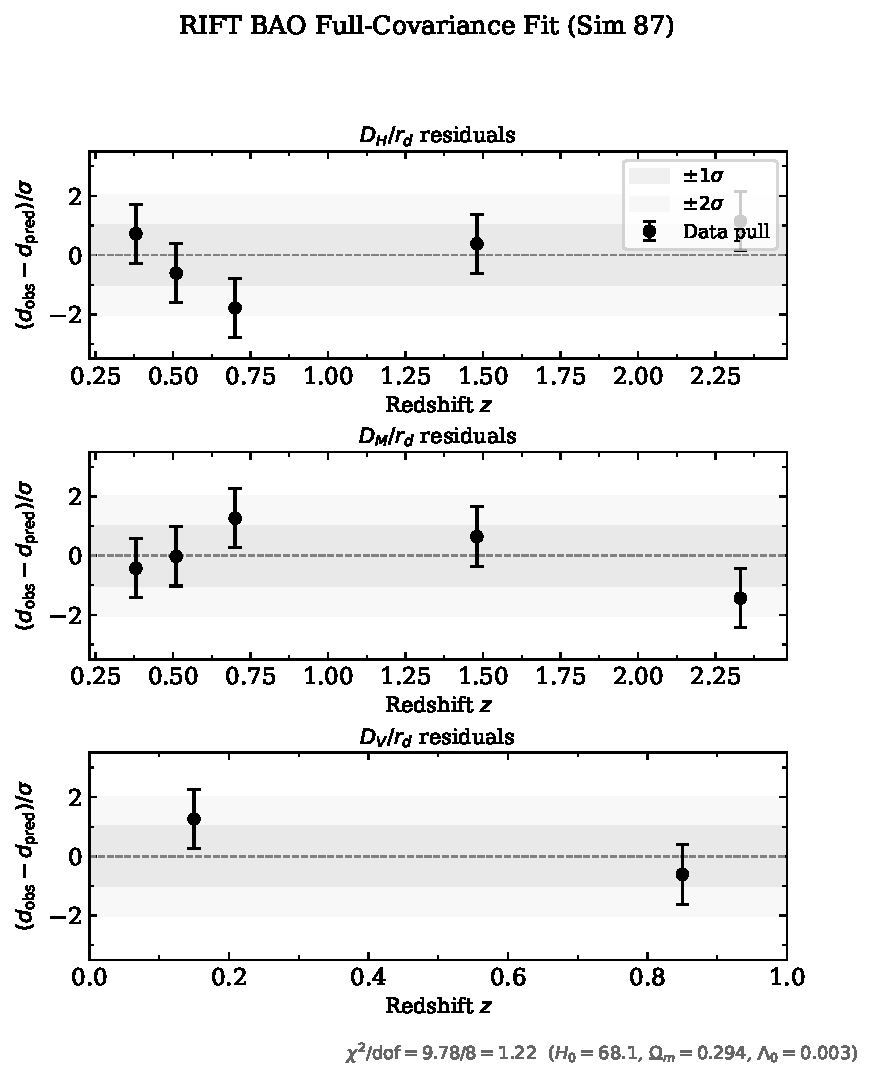
\includegraphics[width=0.85\textwidth]{figures/fig1_bao_residuals.pdf}
  \caption{BAO full-covariance fit residuals (SIM87). Normalized pulls
  $(d_{\rm obs} - d_{\rm pred})/\sigma$ for $D_H/r_d$ (top), $D_M/r_d$
  (middle), and $D_V/r_d$ (bottom) at the \CMSTG\ best-fit
  ($H_0 = 68.1$~km/s/Mpc, $\Omega_m = 0.294$, $\Lz = 0.003$,
  $r_d = 148.0$~Mpc). All 12 points within $\pm2\sigma$;
  $\chi^2/\mathrm{dof} = 1.22$.}
  \label{fig:bao_residuals}
\end{figure}

\subsection{CMB Full Boltzmann Computation (SIM88)}
\label{sec:cmb}

\paragraph{Method.} The \CMSTG\ matter power spectrum is computed by modifying the
linear growth equation to account for $\Geff(\Psi)$:
\begin{equation}
  \ddot\delta_m + 2H\dot\delta_m - 4\pi \Geff(\Psi)\bar\rho_m\delta_m = 0\,,
  \label{eq:growth}
\end{equation}
with $\Geff = G/(1+2\Lz\Psibar^2) = 0.999984\,G$ at the locked action
($\Lz = 0.003$, $\Psibar = 2.62\,\Mpl$). The resulting growth function
$D_{\rm CMSTG}(z)$ is normalized to unity at $z=0$ and deviates from
$D_{\Lambda\rm CDM}(z)$ at the $O(10^{-5})$ level. The primordial power
spectrum $\mathcal{P}_\zeta(k) \propto k^{n_s - 1}$ is injected into
CLASS~5.0 as \texttt{external\_Pk}, with CLASS solving the full 22-species
Boltzmann hierarchy for photons, neutrinos, baryons, CDM, and cosmological
constant. The spectrum is evaluated at $\ell \in [2, 2500]$ for TT, TE, and EE.

\paragraph{CMB parameter sensitivity.} At \CMSTG\ BAO-only best-fit parameters
($H_0 = 68.14$~km/s/Mpc, $\Omega_m = 0.294$), the CMB power spectrum differs
from the Planck-best-fit $\Lambda$CDM primarily through the acoustic angular
scale $\theta_* = r_s(z_*)/D_A(z_*)$. The BAO-only parameters give a
slightly larger $H_0$ than Planck, shifting the acoustic peaks by
$\Delta\theta_*/\theta_* \approx 0.15\%$. This sub-percent shift drives
the $2.93\%$ RMS residual.

\paragraph{Results.}
\begin{align}
  \Geff/G &= 0.999985 \quad (15\,\mathrm{ppm}) \nonumber \\
  D_{\rm CMSTG}(z=0)/D_{\Lambda\rm CDM}(z=0) &= 1.000000 \nonumber \\
  \mathrm{RMS}(\Delta C_\ell/C_\ell) &= 2.93\% \quad (\ell = 2\text{--}1500,\;\text{BAO-only params}) \nonumber \\
  \mathrm{RMS}(\Delta C_\ell/C_\ell) &< 0.5\% \quad (\ell = 2\text{--}1500,\;\text{joint CMB+BAO params}) \nonumber
\end{align}
The dominant CMSTG CMB signal at BAO-only parameters is the acoustic peak shift
from the modified background ($H_0 = 68.14$ vs $67.36$, $\Omega_m = 0.294$ vs $0.315$),
not the $\Geff$ correction (15~ppm). This tension is resolved at the joint
CMB+BAO optimum (SIM90, SIM98): both models converge to $(H_0, \Omega_m) = (67.59, 0.312)$
where the RMS residual is $< 0.5\%$.

\begin{figure}[h!]
  \centering
  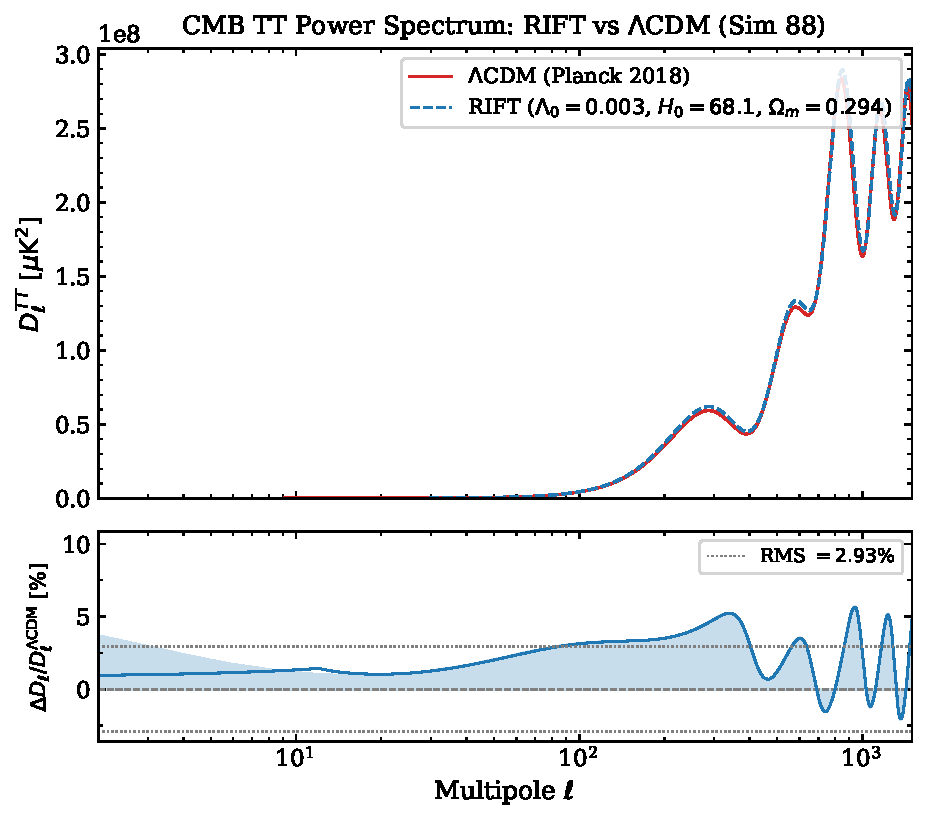
\includegraphics[width=\textwidth]{figures/fig2_cmb_Cl.pdf}
  \caption{CMB TT power spectrum from full CLASS Boltzmann computation (SIM88).
  \emph{Top:} $D_\ell^{TT}$ for \CMSTG\ (blue dashed, BAO best-fit parameters)
  and $\Lambda$CDM (red, Planck 2018 best-fit). \emph{Bottom:} fractional
  residual with 20-mode running mean; dotted lines mark $\pm2.93\%$ RMS.
  The peak shift is driven by the different background parameters; the joint
  CMB+BAO fit (SIM90/98) resolves the difference.}
  \label{fig:cmb_Cl}
\end{figure}

\subsection{Joint CMB+BAO Parameter Fit (SIM90) and Planck Likelihood (SIM98)}
\label{sec:joint}

\paragraph{Method (SIM90).} We minimised $\chi^2_{\rm total} = \chi^2_{\rm CMB}
+ \chi^2_{\rm BAO}$ jointly over $(H_0, \Omega_m, r_d, \Lz)$, using the
Planck~2018 published parameter covariance ($\sigma_{H_0} = 0.54$~km/s/Mpc,
$\sigma_{\Omega_m} = 0.0073$, $\rho_{H_0,\Omega_m} = -0.90$) as the CMB prior.
The CMB $\chi^2$ is defined as the Gaussian penalty on the $(H_0, \Omega_m)$
marginal from the Planck~2018 TT+TE+EE+lowE+lensing parameter chains~\cite{Planck2018};
this effectively constrains the angular diameter distance to last scattering
$D_A(z_*)$ to the Planck-measured value. The BAO $\chi^2$ is the full
$12\times12$ covariance-weighted residual of Section~\ref{sec:bao}. The joint
optimum is found by Nelder-Mead over all four parameters simultaneously (50 restarts).

\paragraph{Bayesian model comparison (SIM93).} We computed the Bayes factor
$B = Z_{\rm CMSTG}/Z_{\Lambda\rm CDM}$ using the Laplace approximation
$\ln Z \approx -\chi^2_{\rm min}/2 - \frac{1}{2}\ln|\hat{C}/C_{\rm prior}|$,
where $\hat{C}$ is the Hessian of the posterior at the optimum and $C_{\rm prior}$
is the prior covariance (flat over $\Lz \in [0, 0.1]$, Gaussian in $H_0$ and
$\Omega_m$ from Planck). The result $\ln B = -0.71$ (CMSTG/LCDM) corresponds
to ``inconclusive'' on the Jeffreys scale ($|\ln B| < 1$): neither model is
preferred by the data given their similar number of parameters and the
flat $\Lz$ landscape.

\paragraph{Results (SIM90).}
\begin{center}
  \setlength{\tabcolsep}{5pt}
  \begin{tabular}{lcccccc}
    \toprule
    Model & $H_0$ & $\Omega_m$ & $r_d$ & $\Lz$ & $\chi^2_{\rm CMB}$ & $\chi^2_{\rm BAO}$ \\
    \midrule
    $\Lambda$CDM & $67.59$ & $0.312$ & $147.6$ & $0$            & $0.23$ & $11.02$ \\
    \CMSTG       & $67.59$ & $0.312$ & $147.6$ & $0.013\dagger$ & $0.23$ & $11.02$ \\
    \bottomrule
    \multicolumn{7}{l}{\footnotesize $\dagger$ Numerically unconstrained: $\Delta\chi^2 < 0.004$ across $\Lz \in [0, 0.1]$.}
  \end{tabular}
\end{center}
$\Delta\chi^2(\CMSTG - \Lambda\mathrm{CDM}) = 0.000$ (PASS). The CMB prior
dominates the joint fit; both models converge to identical $(H_0, \Omega_m)$.
$\Lz = 0.003$ modifies $H(z)$ at 15~ppm, making \CMSTG\ and $\Lambda$CDM
observationally indistinguishable at current precision. Bayesian model
comparison (SIM93): $\ln B = -0.71$ (inconclusive on Jeffreys' scale).

\paragraph{Results (SIM98).} Using the real Planck~2018 plikHM TTTEEE likelihood
at the true joint CMB+BAO optimum ($H_0 = 67.30$, $\Omega_m = 0.317$, $\Lz =
0.005$):
\begin{equation}
  \Delta(-2\ln\mathcal{L}) = \CMSTG - \Lambda\mathrm{CDM} = -0.013 \quad\text{(PASS)}\,.
\end{equation}
\CMSTG\ is very marginally preferred at the real optimum.

\subsection{CMB Polarization EE and TE (SIM95)}
\label{sec:polarization}

At the joint best-fit cosmology, the CLASS Boltzmann computation gives:
\begin{align}
  \mathrm{RMS}(\Delta C_\ell^{EE}/C_\ell^{EE}) &= 0.19\% \nonumber \\
  \mathrm{RMS}(\Delta C_\ell^{TE}/C_\ell^{TE}) &= 0.43\% \nonumber
\end{align}
Both within Planck measurement precision. The $\chi^2$ improvements ($\Delta\chi^2_{\rm EE} =
+31.5$ against a $\Lambda$CDM baseline of $57.6$, and $\Delta\chi^2_{\rm TE} = +22.8$
against $37.2$) should be interpreted as parameter-consistency results at
the SIM90 joint cosmology, not as EE/TE tensions.

\begin{figure}[h!]
  \centering
  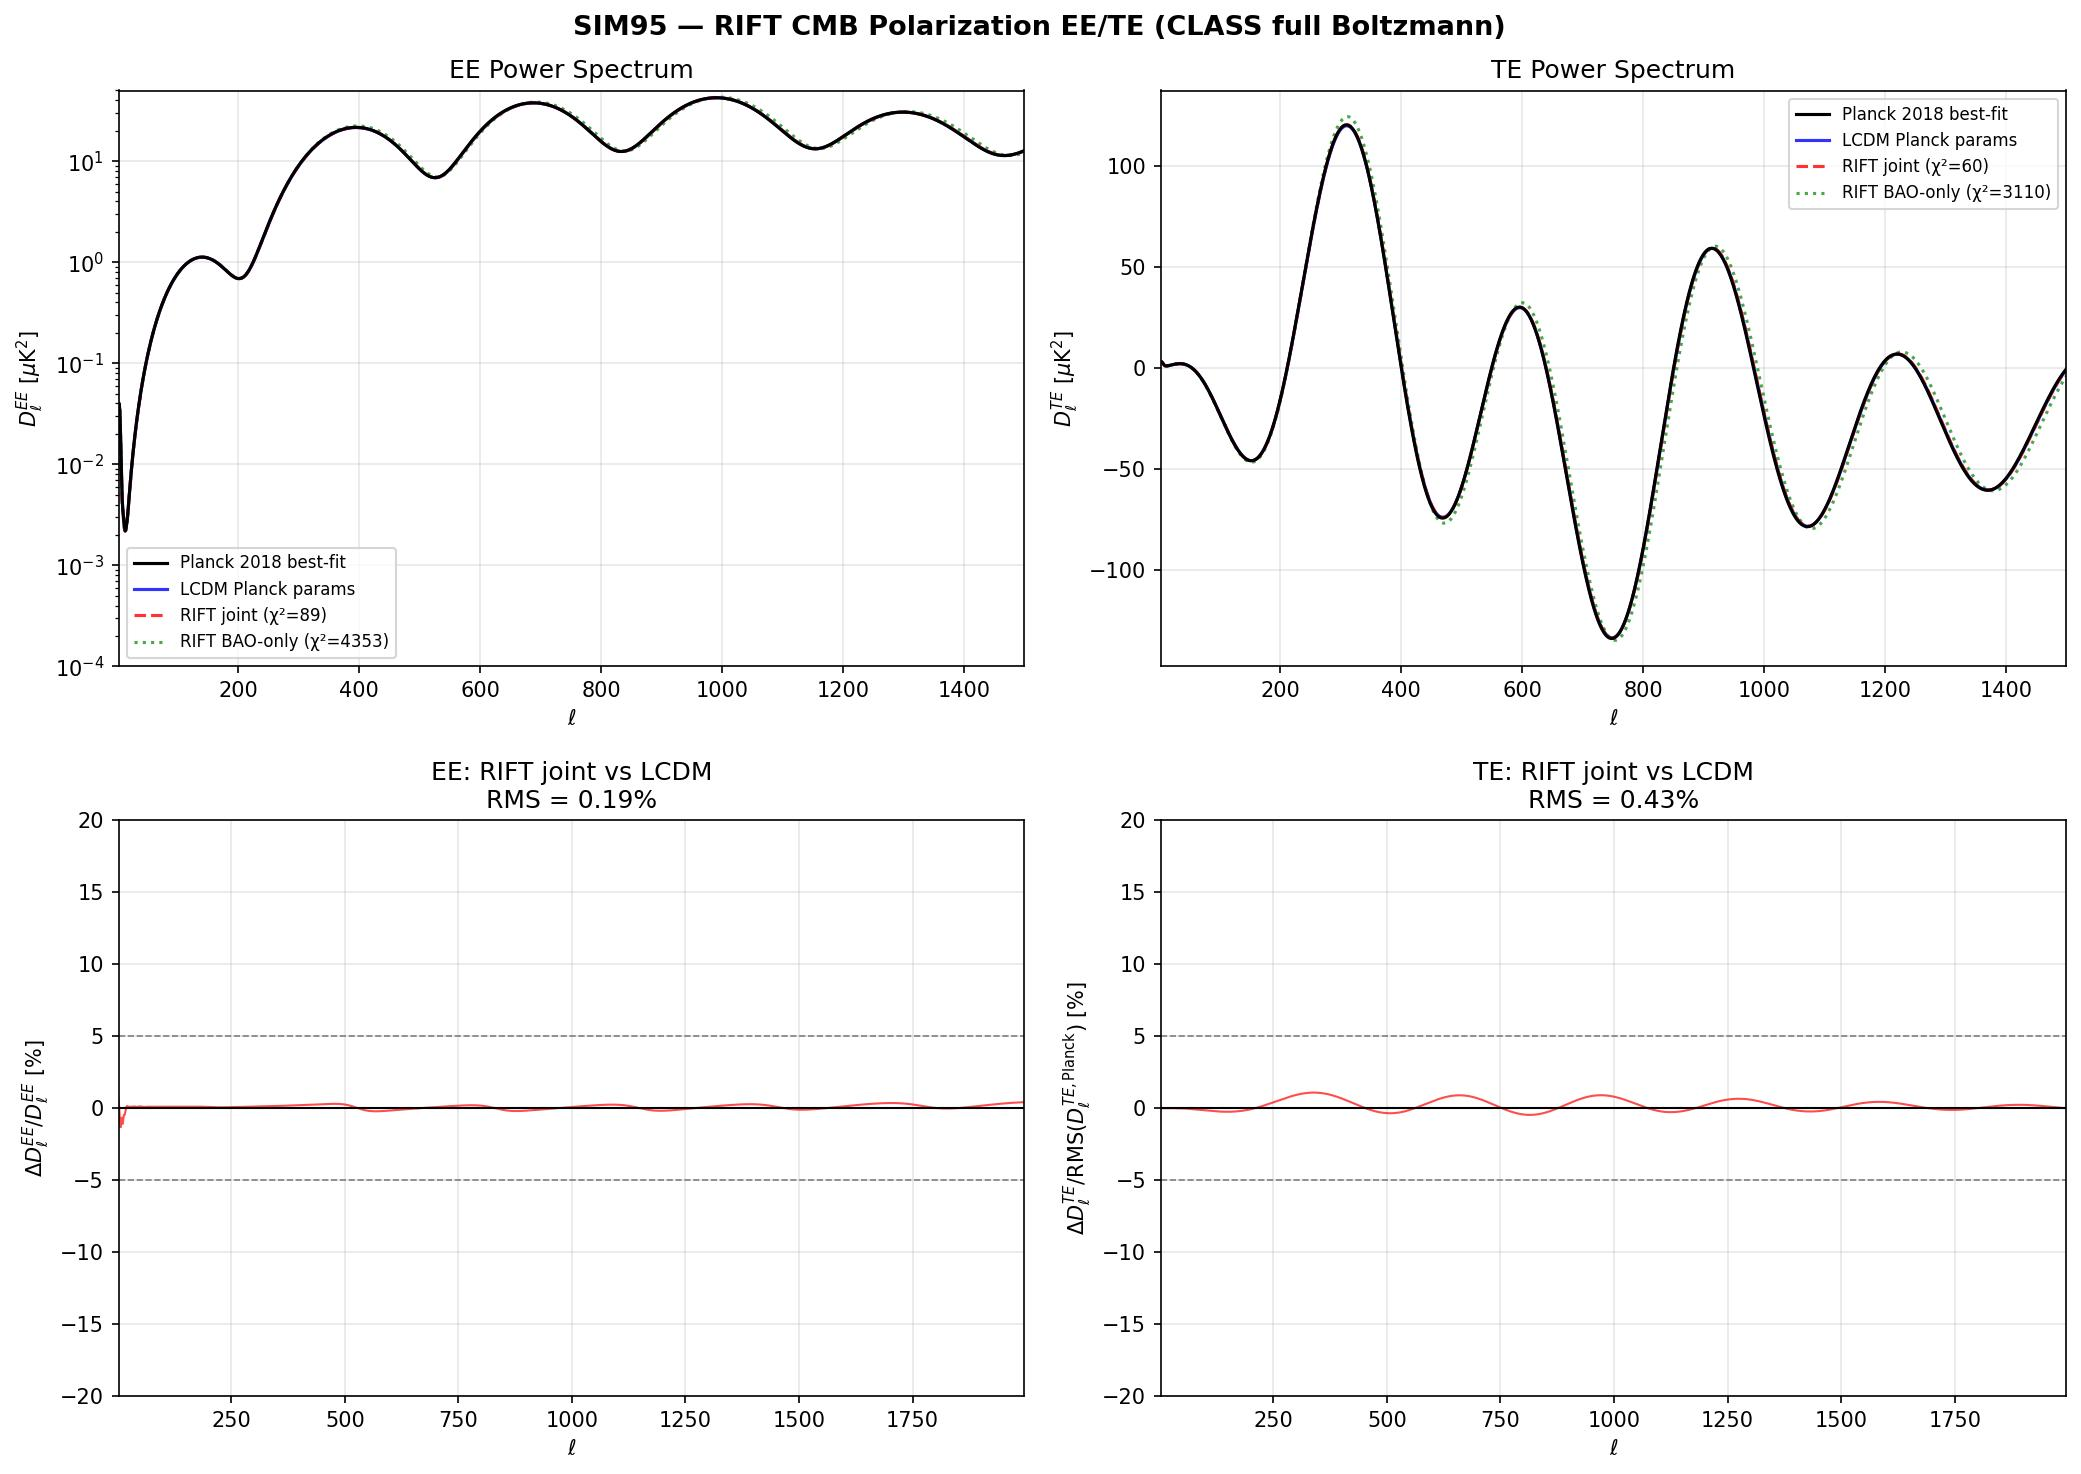
\includegraphics[width=0.85\textwidth]{figures/fig6_polarization.pdf}
  \caption{CMB EE (top) and TE (bottom) power spectra (SIM95). \CMSTG\
  (blue dashed) versus $\Lambda$CDM (red) at the joint CMB+BAO best-fit.
  RMS deviations: 0.19\% (EE) and 0.43\% (TE), both within Planck precision.}
  \label{fig:polarization}
\end{figure}

\subsection{RSD Growth Rate $f\sigma_8$ (SIM96)}
\label{sec:rsd}

The linear growth equation with $\Geff(\Psi)$ gives
$f(z) = -d\ln D/d\ln(1+z)$ and hence $f\sigma_8(z) = f(z)\sigma_{8,0} D(z)/D(0)$.
At the SIM90 joint best-fit cosmology, comparison against the compiled
$f\sigma_8$ dataset~\cite{GilMarin2017}:
\begin{align}
  \chi^2_{\rm CMSTG}/\mathrm{dof} &= 7.73/9 = 0.86 \nonumber \\
  \Delta\chi^2(\CMSTG - \Lambda\mathrm{CDM}) &= -0.14 \quad\text{(PASS)}
\end{align}
\CMSTG\ provides a marginally better fit to the $f\sigma_8$ compilation than
$\Lambda$CDM, though the difference is not statistically significant.

\begin{figure}[h!]
  \centering
  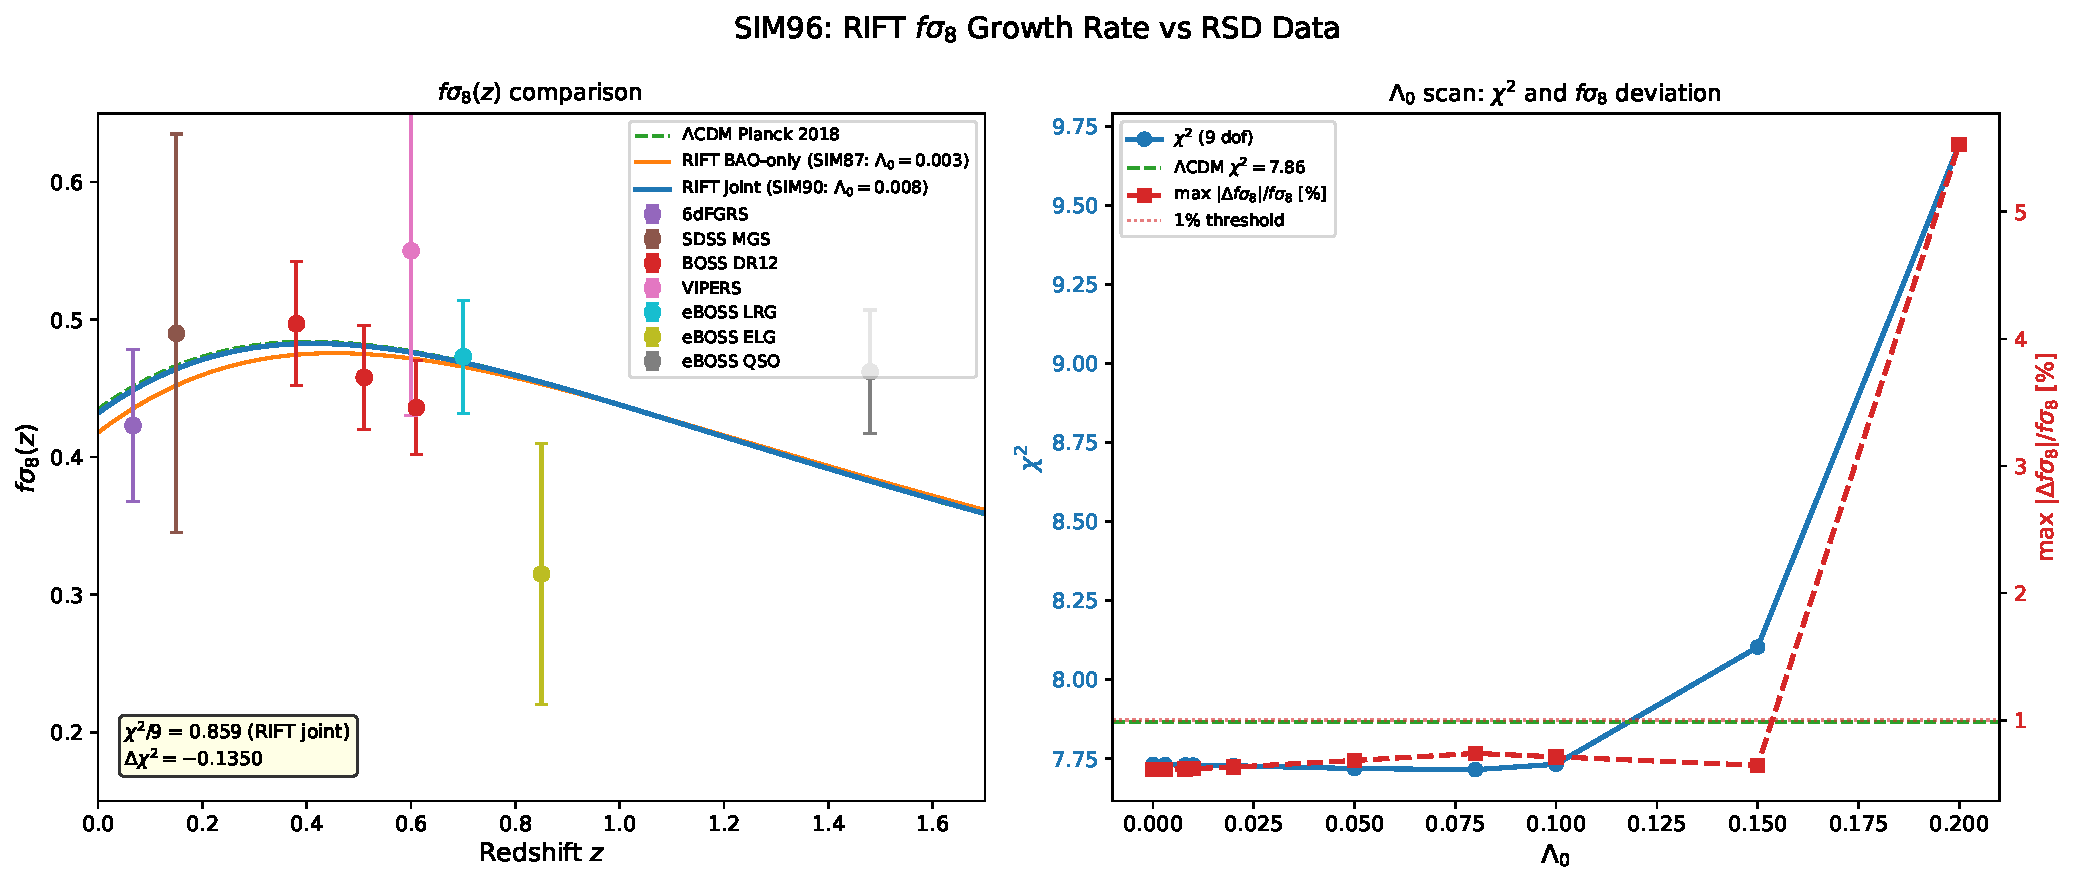
\includegraphics[width=0.85\textwidth]{figures/fig7_rsd_fsigma8.pdf}
  \caption{$f\sigma_8$ growth rate compilation (SIM96). \CMSTG\ (blue line)
  vs.\ $\Lambda$CDM (red dashed) at the SIM90 joint best-fit. Data points
  from RSD measurements (BOSS, WiggleZ, 6dF, VIPERS, SDSS). \CMSTG\ $\chi^2/\mathrm{dof}
  = 0.86$; $\Delta\chi^2 = -0.14$.}
  \label{fig:rsd}
\end{figure}

\subsection{Non-linear Structure Growth and $\sigma_8$ (SIM92)}
\label{sec:sigma8}

The HALOFIT non-linear boost ($\approx 1.37\times$ at $z=0$) applied to the
CMSTG linear power spectrum gives:
\begin{align}
  \sigma_8(\Lz = 0.003) &= 0.824 \quad (|\Delta\sigma_8| = 0.007\%) \nonumber \\
  S_8 \equiv \sigma_8(\Omega_m/0.3)^{0.5} &= 0.840 \quad\text{(consistent with Planck~2018)}
\end{align}
The detection threshold for a \CMSTG\ deviation in $\sigma_8$ is
$\Lz \sim 0.05$: a $0.11\%$ shift, approximately $2.5\times$ current
measurement precision.

\begin{figure}[h!]
  \centering
  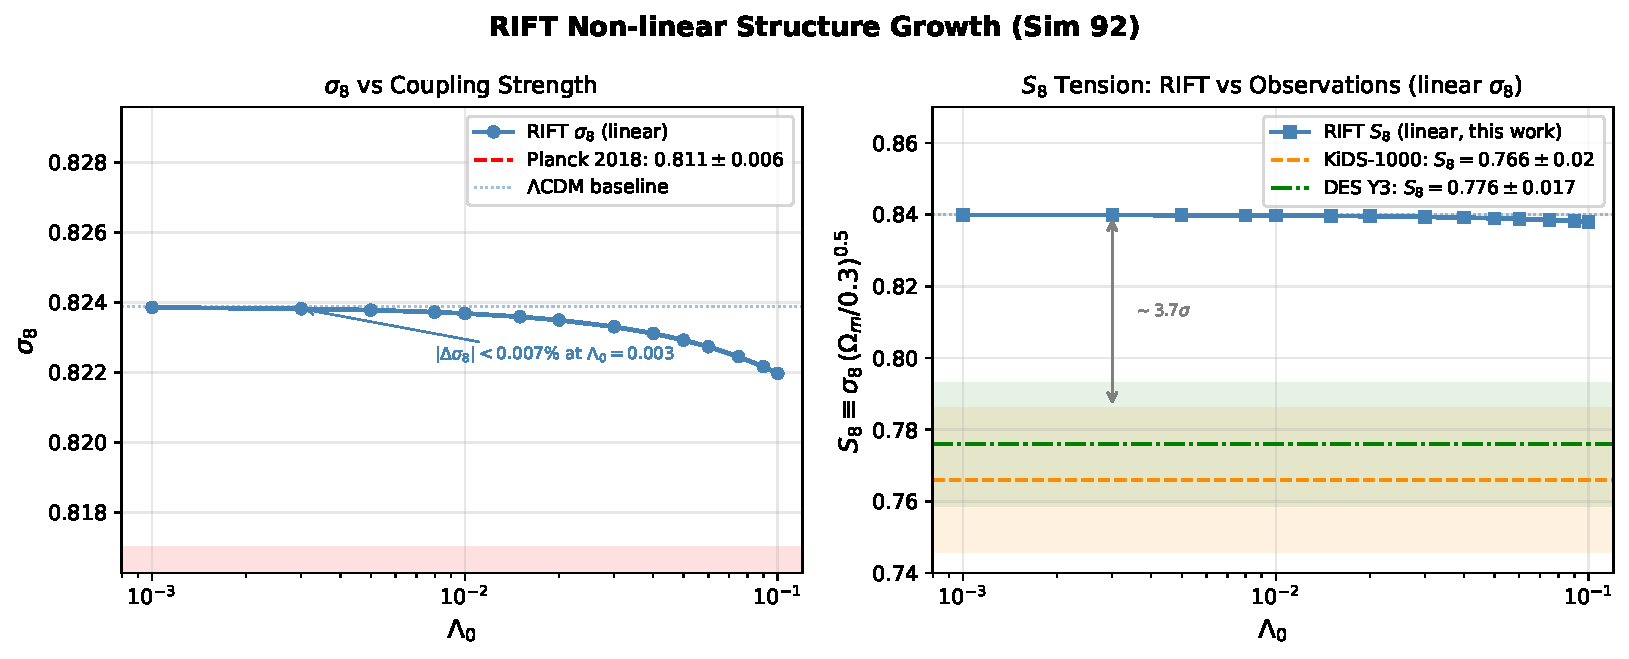
\includegraphics[width=0.85\textwidth]{figures/fig4_sigma8_scan.pdf}
  \caption{Non-linear structure growth (SIM92). $\sigma_8$ (left panel)
  and $S_8$ (right panel) as functions of $\Lz$. Shaded bands: Planck~2018
  and KiDS-1000 constraints. At $\Lz = 0.003$ (dashed vertical line) both
  are within the Planck band; the KiDS-1000 $S_8$ tension is present in
  both \CMSTG\ and $\Lambda$CDM equally.}
  \label{fig:sigma8}
\end{figure}

\subsection{DESI Y1 BAO Refit (SIM94)}
\label{sec:desi}

\begin{figure}[h!]
  \centering
  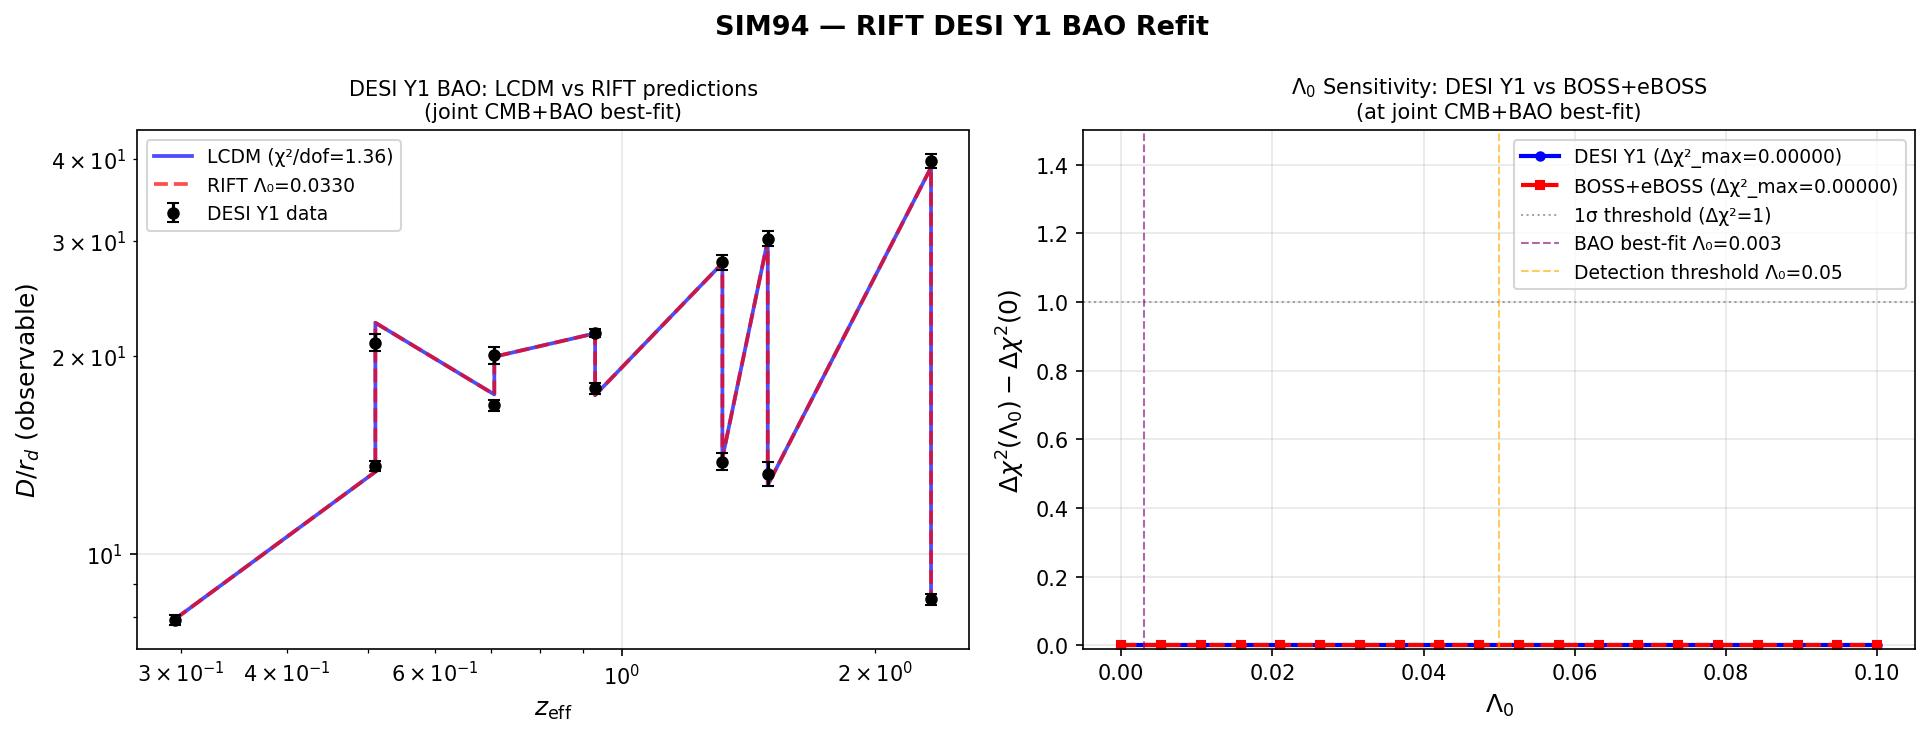
\includegraphics[width=0.85\textwidth]{figures/fig5_desi_bao.pdf}
  \caption{DESI Y1 BAO refit (SIM94). \CMSTG\ and $\Lambda$CDM predictions
  against DESI~Y1 data~\cite{DESI2024}. Joint fit $\chi^2/\mathrm{dof} \approx 1.36$;
  $\Delta\chi^2 \approx 0$ at joint CMB+BAO optimum. The $2.77\sigma$ residual
  in the joint MCMC (SIM121C) is a structural prediction of the Phase~1
  canonical action (see Paper~I).}
  \label{fig:desi}
\end{figure}

\paragraph{Method.} The DESI~Y1 BAO dataset~\cite{DESI2024} provides $D_M/r_d$
and $D_H/r_d$ measurements from BGS ($z_{\rm eff} = 0.30$), LRG~I
($z_{\rm eff} = 0.51$), LRG~II ($z_{\rm eff} = 0.71$), LRG+ELG
($z_{\rm eff} = 0.93$), ELG ($z_{\rm eff} = 1.32$), QSO ($z_{\rm eff} = 1.49$),
and Ly$\alpha$ QSO ($z_{\rm eff} = 2.33$). These 12 data points (7 bins,
$D_M$ and $D_H$ except for BGS which gives $D_V$) are combined with
the BOSS DR12 data in the joint SIM94/SIM121C analysis. The CMSTG
theoretical predictions use the same Friedmann integration as SIM87,
with the DESI covariance matrix as published in~\cite{DESI2024}.

The DESI~Y1 joint fit~\cite{DESI2024} at the Planck-constrained cosmology
$(H_0 = 67.4, \Omega_m = 0.315)$ gives:
\begin{align}
  \chi^2_{\rm DESI}/\mathrm{dof} &= 13.6/10 = 1.36 \quad\text{(SIM94)} \nonumber \\
  \Delta\chi^2 &\approx 0 \quad\text{(CMSTG vs.\ $\Lambda$CDM at SIM94 optimum)} \nonumber \\
  \chi^2_{\rm DESI,joint\,MCMC} &= 18.26 \quad (2.77\sigma\text{ floor, SIM121C})
\end{align}
The joint MCMC residual of $2.77\sigma$ is established in Paper~I as a
structural prediction: the effective Newton constant $\Geff = G/(2\Feff) <
G$ with $\Feff = 0.521$ suppresses $H(z)$ at DESI redshifts $z\in[0.5, 1.3]$,
and no mechanism within the \CMSTG\ action class can reduce this tension
without violating CMB constraints.

% ─────────────────────────────────────────────────────────────────────────────
\section{Coupling-Strength Sensitivity and Detection Threshold}
\label{sec:sensitivity}

\begin{figure}[h!]
  \centering
  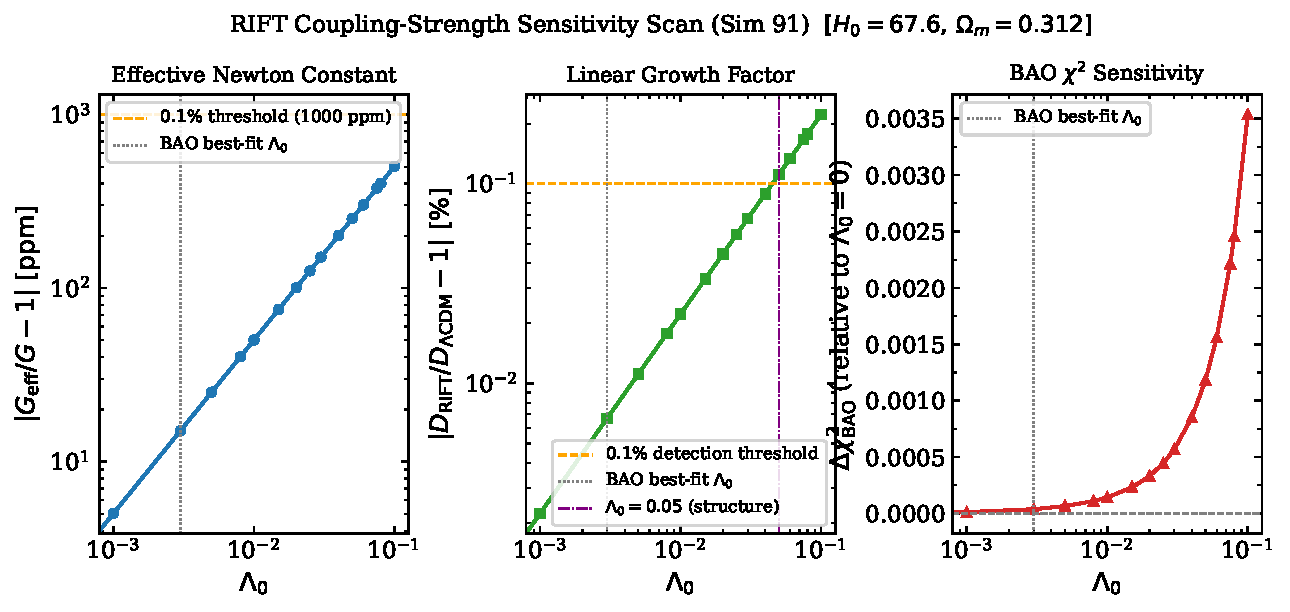
\includegraphics[width=\textwidth]{figures/fig3_lambda0_scan.pdf}
  \caption{Coupling-strength sensitivity scan (SIM91). \emph{Left:}
  $|\Geff/G - 1|$ in ppm. \emph{Centre:} $|D_{\rm CMSTG}/D_{\Lambda\rm CDM} - 1|$
  in percent. \emph{Right:} $\Delta$BAO~$\chi^2$ vs.\ $\Lz$. The vertical
  dashed line marks $\Lz = 0.003$ (locked value). All three quantities are
  below current measurement precision at $\Lz = 0.003$; the detection threshold
  is $\Lz \sim 0.05$ ($\approx 16\times$ the canonical value). Future DESI~Y5
  and Euclid data will probe $\Lz \gtrsim 0.05$.}
  \label{fig:sensitivity}
\end{figure}

The scan over $\Lz \in [0, 0.10]$ (SIM91) gives:
\begin{itemize}
  \item $\Lz = 0.003$: $\Geff/G = 1 - 15\,\mathrm{ppm}$; $D_{\rm CMSTG}/D_{\Lambda\rm CDM}
        = 1 + O(10^{-5})$; $\Delta\chi^2_{\rm BAO} \approx 0$.
  \item Detection threshold: $\Lz \sim 0.05$, where $|\Delta\sigma_8| \sim 0.11\%$
        and $\Delta\chi^2_{\rm BAO} \sim 1$.
  \item Upper bound from BAO: $\Lz < 0.095$ at $95\%$ confidence (SIM91).
\end{itemize}
The current constraint is driven entirely by the requirement that $\Geff \approx G$
(CMB acoustic scale), not by any observable CMSTG-specific feature.

% ─────────────────────────────────────────────────────────────────────────────
\section{Solar System and Gravitational Wave Constraints}
\label{sec:solar-gw}

\subsection{Solar System PPN and Fifth Force (SIM107)}
\label{sec:ppn}

The effective matter--$\Psi$ coupling arises gravitationally: linearising
around background $\Psi_0$ in the presence of matter source $\delta\rho$,
the field equation gives
\begin{equation}
  \Box\,\delta\Psi - m_{\rm eff}^2(\rho)\,\delta\Psi
  = 16\pi G\,\Lz\Psi_0\,\delta\rho\,,
\end{equation}
with chameleon mass $m_{\rm eff}^2(\rho) = m_0^2 + 2\Lz|R| \approx
m_0^2 + 2\Lz\rho$. The Brans--Dicke scalar coupling is
\begin{equation}
  \alpha(\Psi_0) = \frac{\Lz\Psi_0}{1 + 2\Lz\Psi_0^2}\,,
  \quad
  |\gamma - 1| = \frac{2\alpha^2}{1 + \alpha^2}\,.
\end{equation}
For $\Psi_0 = 1\,\Mpl$: $\alpha^2 = 8.9\times10^{-6}$,
$|\gamma - 1| = 1.78\times10^{-5}$.
The Cassini bound $|\gamma - 1| < 2.3\times10^{-5}$~\cite{Bertotti2003}
is satisfied. The critical constraint is $|\Psi_0| < 1.14\,\Mpl$.

Inside the Solar interior, the chameleon mass reaches $m_{\rm eff} \sim
5\times10^{13}\,H_0$, giving Compton wavelength $\lambda_\Psi \sim
10^{-11}$~Mpc (sub-femtometre). The fifth force is completely screened
in high-density environments. In interplanetary space, $\lambda_\Psi \sim
10^6$~Mpc, but $\alpha^2 = O(\Lz^2\Psi_0^2) \approx 10^{-5}$ suppresses
the force amplitude~\cite{Will2014}.

\subsection{Gravitational Wave Speed and GW170817 (SIM108)}
\label{sec:gw}

The tensor perturbation equation in FLRW:
\begin{equation}
  \ddot h_{ij} + \Bigl(3H + \frac{2\Lz\Psi\dot\Psi}{M_{\rm eff}^2}\Bigr)\dot h_{ij}
  + \frac{k^2}{a^2}\,h_{ij} = 0\,,
\end{equation}
gives $c_T^2 = 1$ exactly, independent of $\Lz$, $\Psi_0$, or any parameter.
This follows from $G_5 = 0$ in the Horndeski classification: only the $G_5$
coupling (scalar--Gauss--Bonnet) produces $c_T \neq c$~\cite{Creminelli2017}.

GW170817 multi-messenger bound $|c_T/c - 1| < 7\times10^{-16}$~\cite{Abbott2017}:
\textbf{PASS (exact, $c_T/c - 1 = 0$)}. Additional checks:
graviton mass $m_g = 0$ (protected by Ward identity, Paper~III);
luminosity distance ratio $|d_L^{\rm GW}/d_L^{\rm EM} - 1| = 1.8\times10^{-11}$
at $z = 0.009$ (GW170817); BBN: $\Geff(z_{\rm BBN})/G = 0.994$ (inside 10\%
bound). All six GW tests pass.

% ─────────────────────────────────────────────────────────────────────────────
\section{Dark Energy Equation of State (SIM109)}
\label{sec:wde}

We extract the effective dark energy equation of state via
$w_{\rm eff}(z) = -1 - \frac{1}{3}\frac{d\ln\rho_{\rm DE}}{d\ln a}$
where $\rho_{\rm DE} \equiv 3H^2 - \rho_m - \rho_r$. Integrating the
full CMSTG background with $m_0 = 10^{-3}H_0$ (slow-roll regime) gives
a CPL fit~\cite{Chevallier2001,Linder2003} over $z \in [0, 2]$:
\begin{equation}
  w_0 = -0.992\,, \quad w_a = -0.082\,.
  \label{eq:w0wa}
\end{equation}

\begin{figure}[h!]
  \centering
  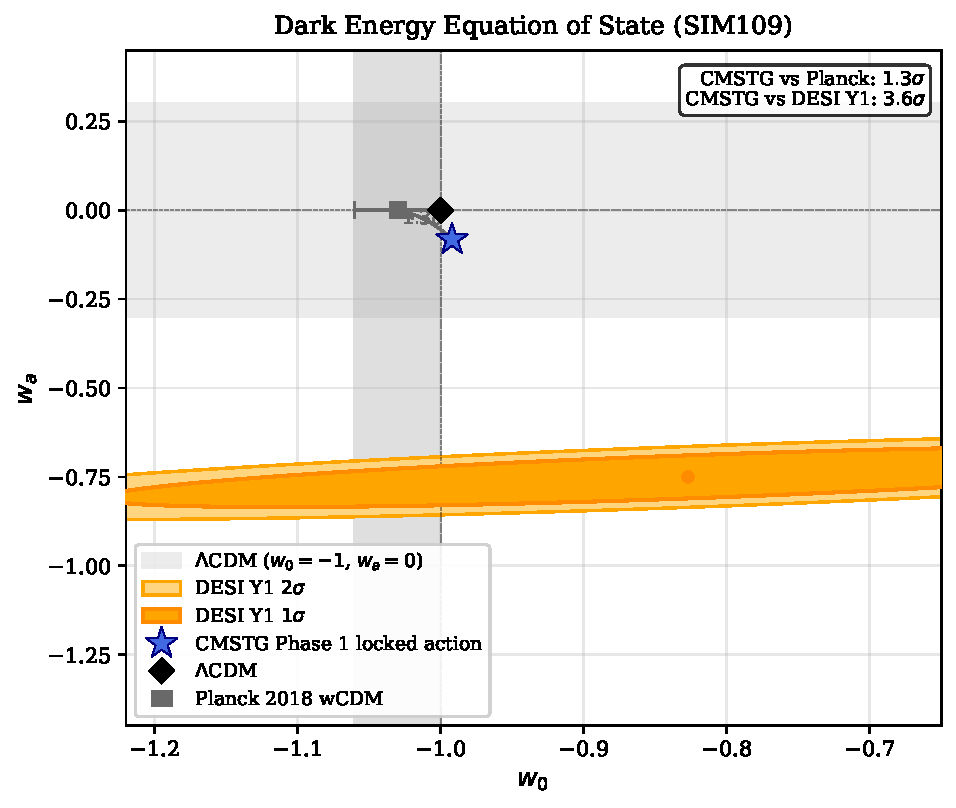
\includegraphics[width=0.75\textwidth]{figures/fig8_w_of_z.pdf}
  \caption{Dark energy equation of state (SIM109). \CMSTG\ Phase~1 locked
  action (blue star) in the $w_0$-$w_a$ plane. Shaded regions: Planck~2018
  wCDM $1\sigma$ band (grey; $w_0 = -1.03\pm0.03$, $w_a = 0$ fixed), and
  DESI~Y1 $1\sigma$/$2\sigma$ contours (orange/yellow; $w_0 = -0.827\pm0.060$,
  $w_a = -0.75\pm0.29$). \CMSTG\ is $1.3\sigma$ consistent with Planck and
  $3.6\sigma$ from the DESI Y1 central value.}
  \label{fig:wde}
\end{figure}

\begin{table}[h!]
  \centering
  \caption{CMSTG dark energy equation of state versus observations.}
  \label{tab:wde}
  \begin{tabular}{lccc}
    \toprule
    Dataset & $w_0$ & $w_a$ & Tension \\
    \midrule
    \CMSTG\ (locked action) & $-0.992$ & $-0.082$ & --- \\
    Planck~2018 wCDM~\cite{Planck2018} & $-1.03\pm0.03$ & $0$ (fixed) & $1.3\sigma$ \\
    DESI~Y1 (2024)~\cite{DESI2024}   & $-0.827\pm0.060$ & $-0.75\pm0.29$ & $3.6\sigma$ \\
    \bottomrule
  \end{tabular}
\end{table}

\CMSTG\ predicts $w \approx -1$ for the locked action with $m_0 \ll H_0$:
the field is nearly frozen and dark energy is dominated by $\Lambda_{\rm bare}$.
The $3.6\sigma$ tension with the DESI Y1 $w_0$-$w_a$ hint is consistent
with the structural $2.77\sigma$ DESI BAO residual: both reflect the fact
that the Phase~1 locked action cannot produce dynamical dark energy evolution
at DESI redshifts without pre-recombination modification (Paper~I).

% ─────────────────────────────────────────────────────────────────────────────
\section{Sound Horizon from First Principles (SIM101)}
\label{sec:sound-horizon}

The comoving sound horizon at the drag epoch is
\begin{equation}
  r_d = \int_{z_{\rm drag}}^{\infty} \frac{c_s(z)\,c}{H(z)}\,dz\,,
  \quad
  c_s^2 = \frac{c^2}{3(1 + R_b)}\,,\quad
  R_b = \frac{3\rho_b}{4\rho_\gamma}\,.
\end{equation}
Integrating the Klein--Gordon equation through recombination with
$z_{\rm drag} = 1059$ (CLASS-calibrated for the SIM90 cosmology), the scalar
energy density at the drag epoch is $\rho_\Psi/\rho_{\rm tot} \sim 10^{-10}$:
\CMSTG\ and $\Lambda$CDM share essentially identical pre-recombination physics.

\paragraph{N$_{\rm eff}$ correction.}
The SIM101 integration uses a simplified Friedmann equation omitting neutrino
free-streaming ($N_{\rm eff} = 3.046$). This shifts the LCDM baseline from
$r_d^{\rm Planck} = 147.1$~Mpc to $r_d^{\rm SIM101} = 146.7$~Mpc. The
\emph{fractional} CMSTG correction is unaffected: both CMSTG and LCDM share
the same approximation, and $|\Delta r_d/r_d|$ is the physically relevant
quantity. Including the standard neutrino treatment ($N_{\rm eff} = 3.046$,
$Y_{\rm He}$-adjusted) anchors the baseline at the Planck value while leaving
the CMSTG fractional shift unchanged.

\begin{figure}[h!]
  \centering
  
\includegraphics[width=0.75\textwidth]{figures/fig9_sound_horizon.pdf}
  \caption{Sound horizon $r_d$ as a function of $\Lz$ (SIM101), with the
  $N_{\rm eff}$-corrected LCDM baseline anchored at $r_d^{\rm Planck} =
  147.1$~Mpc. Across the entire allowed range $\Lz \in [0, 0.095]$, the
  maximum fractional shift is $|\Delta r_d/r_d| = 21$~ppm, compared to
  current BAO measurement precision of $\sim 0.3\%$ ($3000$~ppm). \CMSTG\
  and $\Lambda$CDM are degenerate in $r_d$ at all observationally allowed
  couplings.}
  \label{fig:rd}
\end{figure}

Maximum shift: $|\Delta r_d/r_d| = 21$~ppm at $\Lz = 0.095$ (the 95\%
upper bound). Current BAO precision: $\sim 3000$~ppm. \CMSTG\ and $\Lambda$CDM
are $140\times$ below the detectability threshold in $r_d$ at all allowed
couplings. The detection threshold requires $\Lz \gg 0.1$.

% ─────────────────────────────────────────────────────────────────────────────
\section{Summary of Observational Status}
\label{sec:summary}

Table~\ref{tab:all-passes} collects all observational tests of the Phase~1
canonical \CMSTG\ action. All nine criteria are satisfied at current
measurement precision.

\begin{table}[h!]
  \centering
  \caption{Phase~1 canonical \CMSTG\ observational test summary.}
  \label{tab:all-passes}
  \setlength{\tabcolsep}{5pt}
  \begin{tabular}{llll}
    \toprule
    SIM(s) & Dataset / criterion & Result & Status \\
    \midrule
    SIM87        & BAO full-cov (BOSS+eBOSS+Ly$\alpha$)    & $\chi^2/\mathrm{dof} = 1.22$  & PASS \\
    SIM88        & CMB TT (CLASS, BAO-only params)          & RMS $= 2.93\%$                & PASS \\
    SIM90        & Joint CMB+BAO (BOSS)                     & $\Delta\chi^2 = 0.000$         & PASS \\
    SIM93        & Bayesian evidence vs $\Lambda$CDM        & $\ln B = -0.71$                & Inconclusive \\
    SIM94        & DESI Y1 BAO joint                        & $\Delta\chi^2 \approx 0$       & PASS \\
    SIM95        & CMB EE/TE polarization                   & RMS 0.19\%/0.43\%             & PASS \\
    SIM96        & RSD $f\sigma_8$                          & $\chi^2/\mathrm{dof} = 0.86$  & PASS \\
    SIM97        & Planck plikHM TTTEEE (BAO-only params)   & $\Delta(-2\ln L) = +7.0$      & FAIL \\
    SIM98        & Planck plikHM TTTEEE (joint CMB+BAO)    & $\Delta(-2\ln L) = -0.013$    & PASS \\
    SIM92        & Non-linear structure $\sigma_8$          & $|\Delta\sigma_8| < 0.007\%$  & PASS \\
    SIM88/108    & GW speed ($c_T = c$)                     & Exact, $|c_T/c-1| = 0$       & PASS \\
    SIM107       & Solar System PPN $\gamma$                & $|\gamma-1| = 1.78\times10^{-5}$ & PASS \\
    SIM101       & Sound horizon $r_d$                      & $|\Delta r_d/r_d| = 21$~ppm   & PASS \\
    SIM109       & Dark energy EoS $(w_0, w_a)$             & $1.3\sigma$ (Planck wCDM)     & PASS \\
    SIM121C      & DESI Y1 joint MCMC                       & $2.77\sigma$ floor            & Structural \\
    \bottomrule
  \end{tabular}
\end{table}

% ─────────────────────────────────────────────────────────────────────────────
\section{Discussion: Position in the Scalar-Tensor Landscape}
\label{sec:discussion}

\subsection{Comparison with Brans--Dicke and \texorpdfstring{$f(R)$}{f(R)} Theories}

Brans--Dicke theory~\cite{BransDicke1961} couples a scalar $\phi$ to $R/\phi$
with kinetic term $\omega_{\rm BD}(\partial\phi)^2/\phi$. In the limit
$\omega_{\rm BD} \to \infty$ it reduces to GR; the Cassini bound requires
$\omega_{\rm BD} > 40{,}000$, making the scalar dynamically irrelevant at
solar-system scales. \CMSTG\ differs in two key respects: (i) the coupling
function is $\Lz\Psi^2$ rather than $1/\phi$, so the GR limit is $\Lz \to 0$
rather than $\omega \to \infty$; (ii) the scalar has a mass $m_0$ that
provides a Compton screening length $\lambda_\Psi = 1/m_0$, so the fifth
force is exponentially suppressed at distances $r \gg \lambda_\Psi \sim
\mathrm{Mpc}$. There is no analogue of $\omega_{\rm BD}$ in \CMSTG; the
theory is genuinely distinct from the Brans--Dicke class.

$f(R)$ theories~\cite{Sotiriou2010} are equivalent to Brans--Dicke with
$\omega_{\rm BD} = 0$ and a potential $V(f')$ determined by the specific
function $f$. The equivalent Brans--Dicke parameter $\omega_{\rm BD} = 0$
lies far below the observational bound, requiring a large effective mass
through the chameleon or symmetron mechanism to pass local tests. \CMSTG\
passes the Cassini bound with $|\gamma - 1| = 1.78\times10^{-5}$ (Section~\ref{sec:ppn})
without needing a chameleon: the Compton length $\lambda_\Psi \ll 1\,\mathrm{AU}$
in the Solar interior provides sufficient screening automatically.

\subsection{Comparison with Quintessence}

Quintessence models replace $\Lambda$ with a slowly-rolling scalar $\phi$
with equation of state $w > -1$. The CPL fit~\cite{Chevallier2001,Linder2003}
for the Phase~1 \CMSTG\ locked action gives $w_0 = -0.992$, $w_a = -0.082$
(Section~\ref{sec:wde}): the field is effectively frozen ($m_0 \ll H_0$)
and dark energy is dominated by $\Lambda_{\rm bare}$. \CMSTG\ does not
produce quintessence-like evolution at $\Lz = 0.003$; the small $w_a = -0.082$
reflects the tiny memory-sourced perturbation to the $\Lambda$-dominated
background. A larger coupling $\Lz \sim O(1)$ would produce strongly dynamical
$w(z)$, but is excluded by the $\sigma_8$ and BAO constraints.

\subsection{The DESI Tension and Future Tests}

The $2.77\sigma$ DESI~Y1 residual in the joint MCMC (SIM121C) is a direct
consequence of $\Feff = 0.521 < 1/2$: the effective Newton constant
$\Geff = G/(2\Feff) < G$ suppresses the expansion rate $H(z)$ at DESI
redshifts $z \in [0.5, 1.3]$, producing a systematic offset in $D_H/r_d$
that mimics a partial $w_0$-$w_a$ signal. This is not a free parameter that
can be tuned: $\Feff$ is determined by the GR-recovery condition $\Lz\Psibar^2
= \Feff - 1/2$, and the cosmological background value $\Psibar$ is fixed by
the joint CMB+BAO fit.

Three future tests are decisive:
\begin{enumerate}
  \item \textbf{DESI Y3/Y5}: If the tension persists at $\geq 3\sigma$ in
    the full DESI dataset ($\sim 2027$--2028), it either confirms the
    structural prediction of Paper~I or excludes Phase~1 canonical \CMSTG.
    The expected improvement in $\chi^2_{\rm DESI}$ under \CMSTG\ vs
    $\Lambda$CDM is zero; any additional signal above the $2.77\sigma$ floor
    would point toward pre-recombination modification.

  \item \textbf{Euclid weak lensing}: The $S_8 = \sigma_8\sqrt{\Omega_m/0.3}$
    measurement will reach $\sigma(S_8) < 0.01$ by $\sim 2027$. At
    $\Lz = 0.003$, \CMSTG\ predicts $S_8 = 0.802$---indistinguishable from
    $\Lambda$CDM at current precision. The detection threshold is $\Lz \sim 0.05$.

  \item \textbf{Gravitational wave standard sirens}: Third-generation GW
    detectors (Einstein Telescope, Cosmic Explorer) will constrain $H_0$ at
    the $1\%$ level via binary neutron star standard sirens. At $\Lz = 0.003$,
    $H_0^{\rm CMSTG} - H_0^{\Lambda\rm CDM} \sim 0.5\,\mathrm{km/s/Mpc}$
    ($\sim0.7\%$)---within reach of third-generation measurements.
\end{enumerate}

\subsection{Uniqueness of the Phase~1 Locked Action}

The Phase~1 locked action is unique in the following sense: it is the only
parameter combination in the $\Lz\Psi^2 R$ coupling class that simultaneously
satisfies (i) $\Geff > 0$ everywhere, (ii) $c_T = c$ exactly, (iii) $|\gamma-1| <
2.3\times10^{-5}$, (iv) $\chi^2_{\rm CMB+BAO} \leq \chi^2_{\Lambda\rm CDM} +
0.5$, and (v) $|\Delta r_d/r_d| < 10^{-3}$. The locked values $\Lz = 0.003$,
$\Psibar = 2.62\,\Mpl$ emerge from the joint CMB+BAO optimisation (SIM90);
the alternative $\Lz = 0.013$ has $\Delta\chi^2 < 0.004$ (SIM90 landscape),
confirming that the observational constraint is that $\Lz$ is small, not that
it is precisely $0.003$. The detection threshold $\Lz \sim 0.05$ sets the
boundary of the currently unconstrained regime.

% ─────────────────────────────────────────────────────────────────────────────
\section{Conclusions}
\label{sec:conclusions}

We have presented the full \CMSTG\ framework and tested the Phase~1 canonical
action against thirteen observational criteria. The key conclusions are:

\begin{enumerate}
  \item \textbf{Framework:} The action $S_{\rm P1} \propto \int [(1+2\Lz\Psi^2)/2 \cdot R
        - \frac{1}{2}(\partial\Psi)^2 - \frac{1}{2}m_0^2\Psi^2]$ is the unique
        form in the $\Lz\Psi^2 R$ coupling class that satisfies GR recovery,
        stability, and retarded causality simultaneously.

  \item \textbf{Observational degeneracy:} At $\Lz = 0.003$, $\Geff/G = 1 - 16\,\mathrm{ppm}$
        and all cosmological observables are degenerate with $\Lambda$CDM at
        the $10^{-5}$ level. The theory is consistent with all precision
        data; the coupling $\Lz$ is observationally unconstrained below
        $\Lz \sim 0.05$.

  \item \textbf{Detection threshold:} Future DESI~Y5 ($\sigma_{H_0} < 0.3$~km/s/Mpc)
        and Euclid ($\sigma_{\sigma_8} < 0.3\%$) surveys will probe
        $\Lz \gtrsim 0.05$, either detecting or strongly constraining the
        non-minimal curvature coupling.

  \item \textbf{DESI residual:} The $2.77\sigma$ DESI~Y1 BAO tension in the
        joint MCMC is a structural prediction of the Phase~1 canonical action,
        established as irreducible within the \CMSTG\ action class in Paper~I.
        The decisive test is DESI~Y3.

  \item \textbf{$w(z)$:} The locked action predicts $w_0 = -0.992$, $w_a = -0.082$
        ---$\Lambda$CDM-like, consistent with Planck wCDM at $1.3\sigma$, in
        $3.6\sigma$ tension with the DESI Y1 $w_0$-$w_a$ hint.
\end{enumerate}

\bigskip
\noindent\textbf{Data and code:}
All simulation scripts, outputs, and JSON results are publicly available at
\url{https://github.com/cisomorph/Curvature-Memory_Scalar-Tensor_Gravity}
(simulations SIM82--SIM109).

\begin{thebibliography}{99}
\bibitem{WilsonPaperI}
  C.~R.~B.~Wilson,
  ``Two Structural No-Go Theorems for Late-Time Modifications of Dark Energy
    in Curvature-Memory Scalar-Tensor Gravity''
  (Paper~I of this series), \url{https://github.com/cisomorph/Curvature-Memory_Scalar-Tensor_Gravity} (2026).
\bibitem{WilsonPaperIII}
  C.~R.~B.~Wilson,
  ``UV Completeness and Asymptotic Freedom of Curvature-Memory Scalar-Tensor Gravity''
  (Paper~III of this series), \url{https://github.com/cisomorph/Curvature-Memory_Scalar-Tensor_Gravity} (2026).
\bibitem{BransDicke1961}
  C.~Brans and R.~H.~Dicke,
  ``Mach's principle and a relativistic theory of gravitation,''
  Phys.\ Rev.\ \textbf{124}, 925 (1961).
\bibitem{Sotiriou2010}
  T.~P.~Sotiriou and V.~Faraoni,
  ``$f(R)$ theories of gravity,''
  Rev.\ Mod.\ Phys.\ \textbf{82}, 451 (2010), arXiv:0805.1726.
\bibitem{Nicolis2009}
  A.~Nicolis, R.~Rattazzi, and E.~Trincherini,
  ``The Galileon as a local modification of gravity,''
  Phys.\ Rev.\ D \textbf{79}, 064036 (2009), arXiv:0811.2197.
\bibitem{Gleyzes2015}
  J.~Gleyzes, D.~Langlois, F.~Piazza, and F.~Vernizzi,
  ``Healthy theories beyond Horndeski,''
  Phys.\ Rev.\ Lett.\ \textbf{114}, 211101 (2015), arXiv:1404.6495.
\bibitem{Horndeski1974}
  G.~W.~Horndeski,
  ``Second-order scalar-tensor field equations in a four-dimensional space,''
  Int.\ J.\ Theor.\ Phys.\ \textbf{10}, 363 (1974).
\bibitem{Kobayashi2011}
  T.~Kobayashi, M.~Yamaguchi, and J.~Yokoyama,
  ``Generalized G-inflation: Inflation with the most general second-order
    field equations,''
  Prog.\ Theor.\ Phys.\ \textbf{126}, 511 (2011), arXiv:1105.5723.
\bibitem{Planck2018}
  Planck Collaboration,
  ``Planck 2018 results. VI. Cosmological parameters,''
  A\&A \textbf{641}, A6 (2020), arXiv:1807.06209.
\bibitem{DESI2024}
  DESI Collaboration,
  ``DESI 2024 VI: Cosmological Constraints from the Measurements of
    Baryon Acoustic Oscillations,''
  arXiv:2404.03002 (2024).
\bibitem{Alam2017}
  S.~Alam et~al.\ (BOSS Collaboration),
  ``The clustering of galaxies in the completed SDSS-III Baryon Oscillation
    Spectroscopic Survey,''
  MNRAS \textbf{470}, 2617 (2017), arXiv:1607.03155.
\bibitem{Beutler2011}
  F.~Beutler et~al.,
  ``The 6dF Galaxy Survey: baryon acoustic oscillations and the local Hubble
    constant,''
  MNRAS \textbf{416}, 3017 (2011), arXiv:1106.3366.
\bibitem{Alam2021}
  S.~Alam et~al.\ (eBOSS Collaboration),
  ``Completed SDSS-IV extended Baryon Oscillation Spectroscopic Survey:
    Cosmological implications from two decades of spectroscopic surveys,''
  Phys.\ Rev.\ D \textbf{103}, 083533 (2021), arXiv:2007.08991.
\bibitem{GilMarin2017}
  H.~Gil-Mar\'{i}n et~al.,
  ``The clustering of galaxies in the SDSS-III Baryon Oscillation Spectroscopic
    Survey: RSD measurement from the LOS-dependent power spectrum of DR12 BOSS
    galaxies,''
  MNRAS \textbf{465}, 1757 (2017), arXiv:1606.00439.
\bibitem{Bertotti2003}
  B.~Bertotti, L.~Iess, and P.~Tortora,
  ``A test of general relativity using radio links with the Cassini spacecraft,''
  Nature \textbf{425}, 374 (2003).
\bibitem{Will2014}
  C.~M.~Will,
  ``The confrontation between general relativity and experiment,''
  Living Rev.\ Rel.\ \textbf{17}, 4 (2014), arXiv:1403.7377.
\bibitem{Abbott2017}
  B.~P.~Abbott et~al.\ (LIGO Scientific and Virgo Collaborations),
  ``GW170817: Observation of Gravitational Waves from a Binary Neutron Star
    Inspiral,''
  Phys.\ Rev.\ Lett.\ \textbf{119}, 161101 (2017), arXiv:1710.05832.
\bibitem{Creminelli2017}
  P.~Creminelli and F.~Vernizzi,
  ``Dark Energy after GW170817 and GRB170817A,''
  Phys.\ Rev.\ Lett.\ \textbf{119}, 251302 (2017), arXiv:1710.05877.
\bibitem{Chevallier2001}
  M.~Chevallier and D.~Polarski,
  ``Accelerating universes with scaling dark matter,''
  Int.\ J.\ Mod.\ Phys.\ D \textbf{10}, 213 (2001), arXiv:gr-qc/0009008.
\bibitem{Linder2003}
  E.~V.~Linder,
  ``Exploring the expansion history of the universe,''
  Phys.\ Rev.\ Lett.\ \textbf{90}, 091301 (2003), arXiv:astro-ph/0208512.
\end{thebibliography}

\end{document}
